本講では、アルゴリズムと共にプログラミングを構築する上で非常に重要な要素となるデータ構造について述べる。いくつかのプログラミング言語のチーフデザイナーとして世界的に知られているNiklaus Wirthは、自著のタイトルを"Algorithms+Data Structures=Program"\footnote{邦訳は「アルゴリズムとデータ構造」(浦 昭二他訳、近代科学社、1990)}とし、データ構造の重要性をタイトルからもわかるようにしたとされる。同書は情報科学の世界の古典的名著とされるが、今なお学べる所が多い本であり、これは同時に、データ構造の重要性が古今変わっていないことを示しているともいえよう。
\\ \\ 
なお、ここからの3講はC言語の文法ではなく、これまでの文法を用いて実装できる「応用例」を示す。コードが少なくなり、理論説明が多くなるが、これらの実装を自力で行ったり姉妹書の「実習編」を用いたりして、実際に動かしてみていただきたい。
\section{データ構造とは}
多数のデータを扱うとき、これまでに学んできたデータ型の中では配列や構造体を使うだろう。だが、これら単体ではデータ間の適切な関係を表すことができるとは言い難い。たとえば配列だけでは、頻繁に末尾以外への挿入/削除が起こるような処理は時間がかかってしまうため、別の整理方法を考えなくてはならない。このような「多数のデータを組織的に扱うための整理の方法」を\textbf{データ構造}\index{でーたこうぞう@データ構造}(data structure)と呼ぶ。
\\ \\ 
本講では、基本的なデータ構造のいくつかを扱い、プログラミングでの実装の幅を広げていく。なお、データ構造はここに挙げたものがすべてではなく、まだまだ多くのものがある。それ故、より多くを学びたい人は、他の参考書により学んでいただきたい。

\section{基本的なデータ構造}
まず、スタック・キューという、データ構造の最初に学ぶ「定番」を学ぼう。
\subsection{スタック}
\textbf{スタック}\index{すたっく@スタック}(stack)は棚とも表現されるデータ構造である。この構造は\textbf{FILO}\index{FILO}(First In Last Out)あるいは\textbf{LIFO}\index{LIFO}(Last In First Out)などと形容され、「最初にこの構造に入ったものが最後に出てくる」ないし「最後にこの構造に入ったものが最初に出てくる」構造である。

具体的には、スーパーのかごを思い浮かべるとよいだろう。スーパーのかごが山積みになっているとき、必要になればその上側からかごを取る。逆に、必要なくなったらかごを一番上に返す。この「山積み」がスタックである。
\\ \\ 
「スタック」というと、メモリ領域にも「スタック領域」があった。そして、たとえば再帰処理のメモリの様子を見てみると、確かに「後側に開かれた関数が先に返却値を返す」というスタック構造になっていた。このことからわかるとおり、スタックは再帰処理を用いて代替できる場合もあるし、組み合わせると便利な場合も多い。

では、実際にスタックを用いてみよう。ここでは、スタックを使って回文を判定するプログラムを作ってみよう。
\begin{boxnote}
\begin{multicols}{2}
\minisec{回文の判定}
スタックを用いて、1000文字以下の文字列の回文を判定するプログラムを作成する。ここで入力される文字列は英小文字のみからなるものとする。
\minisec{解説}
回文の判定そのものはスタックを用いなくとも実装可能である(先に述べた「再帰処理による代替」も可能である)。だが、ここであげる方法を応用すると、文字列解釈の際の括弧の対応なども実装できるので、回文はその基礎として組むとよい。

ここで用いたスタックは、擬似的にその動作を模倣するものであるが、動作概要をつかむには十分だろう。
\begin{lstlisting}[caption=回文判定(スタック利用),label=program13_1]
#include<stdio.h>
#include<string.h>

int main(void){
  char str[1024],stack[512];
  int i,j,l,flg=0;

  scanf("%1000s%*c",str);
  l=strlen(str);
  for(i=0;i<l/2;i++)
    stack[i]=str[i];
  for(j=l/2+l%2;j<l;j++){
    if(str[j]!=stack[--i]){
      flg=0;
      break;
    }
    flg=1;
  }
  puts(flg?"YES":"NO");
  return 0;
}
\end{lstlisting}
\end{multicols}
\end{boxnote}

リスト\ref{program13_1}では、$l$.10-11でスタックに文字を積み、$l$.12-13でLIFOの順に文字を取り出していることがわかるだろう。

ここでは擬似的なものとしたが、実際には、スタックに要素を積むための関数と、スタックから要素を出す関数、記憶領域の3つを用意するのが一般的である。

\subsection{キュー}
\textbf{キュー}\index{きゅー@キュー}(queue)とは、待ち行列とも表現されるデータ構造で、スタックに対し\textbf{FIFO}\index{FIFO}(First In First Out)ないし\textbf{LILO}\index{LILO}(Last In Last Out)と形容される。この形容からわかるとおり「最初にこの構造に入ったものが最初に出てくる」「最後にこの構造に入ったものが最後に出てくる」構造である。

同じくスーパーでたとえるなら、こちらはレジの行列(待ち行列)であろう。ある一つのレジでは、先に並んだ人が先に会計を済ませる。この行列こそキューである。
\\ \\ 
それでは、実際にキューを用いた例を見てみることとしよう。
\begin{boxnote}
\begin{multicols}{2}
\minisec{キューを用いたHonorの方法}
(1次以上の)多項式の次数、各次の係数が入力されるとき、区間[-10,10]で0.125刻みで多項式を計算し、出力するプログラムを作成する。
\minisec{解説}
Honorの方法は多項式の計算を高速化する方法である。3次多項式の場合
\[
a_3x^3+a_2x^2+a_1x+a_0
\]
を順に計算すると掛け算6回、足し算3回が必要になる。だが、これを
\[
\left(\left(a_3x+a_2\right)x+a_1\right)x+a_0
\]
として計算すると、掛け算3回、足し算3回になり、計算回数が減る。多項式を幾度も計算する場合などにはこの違いがばかにならなくなってくるので、普段の計算でもこの方法を使う癖をつけておこう(その場合、キューを使わなくてもよいことも多い)。

なお、先のスタックと同じく、これも動作を理解するための擬似的な実装である。
\begin{lstlisting}[caption=Honorの方法(キュー利用),label=program13_2]
#include<stdio.h>

double func(double x,double queue[],int n);

int main(void){
  int n,i;
  double coef[128],x;
  scanf("%d",&n);
  for(i=0;i<=n;i++)
    scanf("%lf",&coef[i]);
  
  for(i=0;i<=160;i++){
    x=0.125*i-10;
    printf("%.3f\t%f\n",x,func(x,coef,n));
  }
  return 0;
}

double func(double x,double queue[],int n){
  double tmp=queue[0]*x+queue[1];
  int i;
  for(i=2;i<=n;i++){
    tmp*=x;
    tmp+=queue[i];
  }
  return tmp;
}
\end{lstlisting}
\end{multicols}
\end{boxnote}

リスト\ref{program13_2}において、$l$.9-10の入力はキューへのインプットである。そして、これを前から使っているのは関数\verb|func|であり、計算が前側から行われている点に注目されたい。

キューの実装についても、スタック同様、キューに要素を入れるための関数と、キューから要素を出す関数、記憶領域の3つを用意するのが一般的である。
\\ \\ 
なお、ここでは実装しなかったが、キューの中が常にソートされた状態であり、昇順/降順に出ていくものを\textbf{プライオリティーキュー}\index{ぷらいおりてぃーきゅー@プライオリティーキュー}(Priority Queue)と呼ぶ。また、両端から挿入/取り出しが可能なキューもあり、これは\textbf{両端キュー}\index{りょうたんきゅー@両端キュー}(double-ended queue)ないし\textbf{デック}\index{でっく@デック}(deque)と呼ばれる。興味があれば調べてみていただきたい\footnote{これらのデータ構造の利用については、「プログラミングコンテストチャレンジブック」(秋葉,岩田,北川 2010 マイナビ)に詳しい。}。

\section{リスト}
\textbf{リスト}\index{りすと@リスト}(list)は\textbf{リンクリスト}\index{りんくりすと@リンクリスト|see{リスト}}(linked-list)とも呼ばれるデータ構造で、データと順序を持つ。配列との違いとして、配列はメモリ上に整然と並んでいるのに対し、リンクリストはポインタを用いて順番を示し、これにより挿入/削除を簡単にしたものである。
\subsection{片方向リスト}
リストは、データ部と次のデータを示すポインタからなる\textbf{自己参照構造体}\index{じこさんしょうこうぞうたい@自己参照構造体}(self-referential structure)を用いて実装することが多い。自己参照構造体は、次のように定義できる。
\begin{itembox}[l]{自己参照構造体の定義}
自己参照構造体を定義する場合、自身へのポインタをメンバに持たせ
\begin{code}
struct tag{
  type member;
     :
  struct tag *next;
};
\end{code}
のように行う。
\end{itembox}

ここで説明した自己参照構造体のように、次の要素を示すポインタとデータ部からなる構造体を定義し、これにより「次は何か」を示して並べたリストを\textbf{片方向リスト}\index{かたほうこうりすと@片方向リスト}(singly-linked list)と呼ぶ。図\ref{Singly}に片方向リストのイメージを示す。
\begin{figure}[htb]
\centering
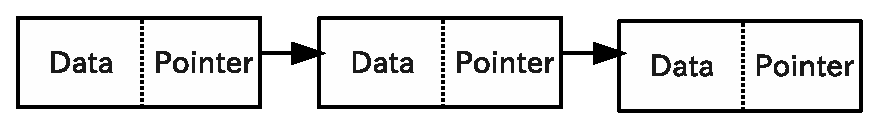
\includegraphics[width=0.75\linewidth,keepaspectratio]{fig13_1.eps}
\caption{片方向リスト}\label{Singly}
\end{figure}

自己参照構造体を複数個用意した後、先頭となるものをひとつ定める。そして、順序付けをポインタを用いて行う。最後の要素のポインタをNULLポインタか先頭要素にしておけば、ターミネータとなる。なお、最後の要素のポインタをNULLにしたものは\textbf{線形リスト}\index{せんけいりすと@線形リスト}(liniarly-linked list)と、先頭要素へのポインタにしたものは\textbf{循環リスト}\index{じゅんかんりすと@循環リスト}(circularly-linked list)と呼ばれている。

\minisec{リストの特徴}
リストに要素を挿入したり、リストから要素を削除するときには、ポインタ部を書き換えることで実現できる。そのため、配列のように多数の要素の書き換えを行う必要がない。これはリストの利点の一つである。

その一方で、メモリ上に連続に配置されているわけではなく、要素番号を用いたアクセスなどができない(ある要素を見つけるために先頭からたどっていく必要がある)ため、配列に比べてアクセスにかかる時間が長くなる。

以上のことからわかるとおり、リストは配列に対し、要素の増減に強く、アクセスに弱いという事になる。そのため、よく増減するようなデータを扱う際などに使うと良い。また、リストはこの後に学ぶグラフのうち、単連結有向グラフの一種でもあるため、グラフの基礎としても使うことができるだろう。
  
\subsection{双方向リスト}
先に学んだ片方向リストでは、次の要素を参照するのは容易であるが、1つ前の要素を参照するのは大変である。そこで、参照のためのポインタを2つに増やし、「次の要素を指すポインタ」と「前の要素を指すポインタ」を準備してやれば、前の要素を参照するのが簡単になるだろう。このように、次の要素と前の要素の両方の参照を持つリストを\textbf{双方向リスト}\index{そうほうこうりすと@双方向リスト}(doubly-linked list)と呼ぶ。図\ref{Doubly}に双方向リストのイメージを示す。
\begin{figure}[htb]
\centering
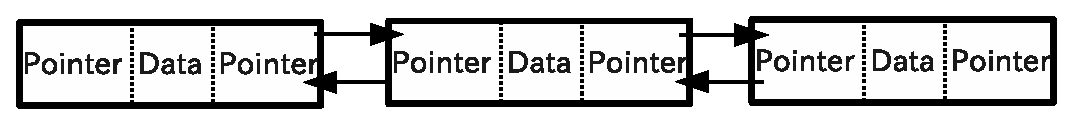
\includegraphics[width=0.95\linewidth,keepaspectratio]{fig13_2.eps}
\caption{双方向リスト}\label{Doubly}
\end{figure}

双方向リストは片方向リストに比べて要素間の行き来が簡単であり、挿入/削除などの容易さもほとんど変わりない。そのため、リストを使う必要性が出てきた場合には双方向リストを使うほうが楽な場合が多いだろう。

\subsection{ループのチェック}
リストにおいて要素間にループがあるかどうかを調べる必要が出てきた時、どのように行えばよいだろうか。片方向リストを例に考えてみよう。
\\ \\ 
一つには、通った要素のログをとっておき、それを参照するという方法がある。だが、これは随分余分にメモリ領域を食ってしまう。あるいは、通った要素に対して、「通ったかどうかのフラグ」をつけ、それが既にオンになっているかどうかをチェックする、という方法もあろう。しかし、これだと、循環のチェック後にフラグをリセットするなどの手間がかかるし、何よりリストに用いた構造体を変更しなければならない(あるいは、リストに用いた構造体をネストとして持つ構造体を作らなければならない)。これらの煩わしい手段を何とかして回避できないものか。

よく知られている方法として、2つのポインタを使う方法がある。リストに用いられている構造体を指すポインタを用意し、共に最初は先頭要素を指しておくものとする。それから、片方のポインタは1つずつ、他方のポインタは2つずつ要素をすすめていく。すると、適切に作られた線形リストならば後者のポインタが先にNULLポインタになるはずである。これがNULLポインタにならず、途中で2つのポインタが出会ってしまう(同じ値を持つ)ようであれば、リストのループが検出されたことになる。この方法は循環リストに使えないように思えるが、循環リストであれば2つのポインタが再び出会う時は先頭要素であるはずである。そのため、この方法を用いればリストが適切に構築されているかどうか、簡単にチェックすることができるのである。

\section{木(Tree)構造}
\textbf{木}\index{き@木}(tree)構造は、「前(親)の要素をひとつだけ持ち、次(子)の要素を複数持つことができる構造」である。各要素のことを\textbf{ノード}\index{のーど@ノード}(node)と呼ぶ。例えば、会社の部署やファイル・ディレクトリの構造などが木構造である。但し、1つの木構造には唯一の「親ノードを持たないノード」が存在し、これを\textbf{根}\index{ね@根}(root)と呼ぶ。逆に、子を持たないノードは\textbf{葉}\index{は@葉}(leaf)と呼ばれる。また、親ノードと子ノードを結ぶ線を\textbf{枝}\index{えだ@枝}(branch)と呼ぶ。図\ref{tree}に木の例を示す。

\begin{figure}[htb]
\centering
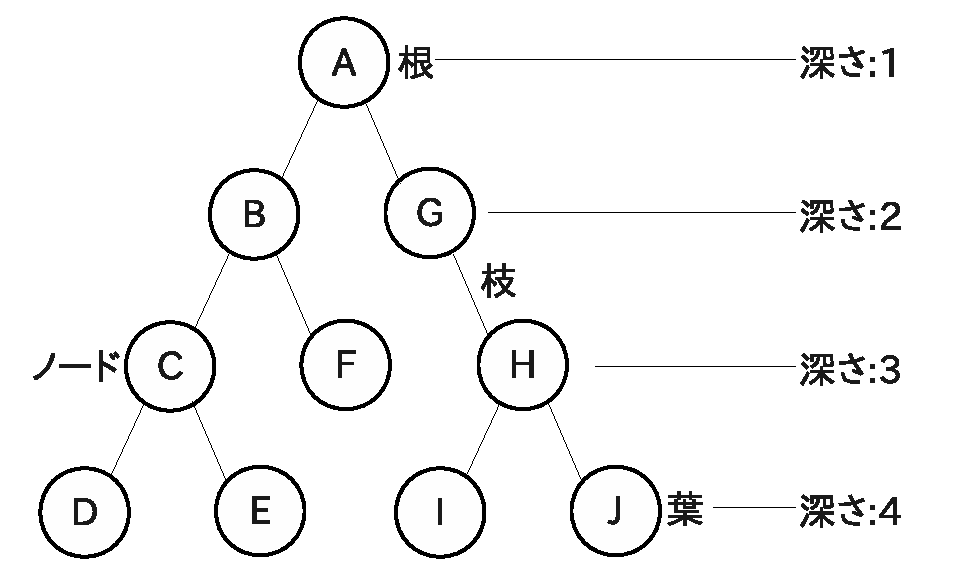
\includegraphics[width=0.8\linewidth,keepaspectratio]{fig13_3.eps}
\caption{木(二分木)の例}\label{tree}
\end{figure}

図\ref{tree}において、「深さ」と記したのは、根を1としてそこから何本の枝でいけるかを足したものであり、そのノードがどの階層に属するかを示している。また、この図を見るとわかるとおり、木はその一部分を取り出しても(例えば、ノードB及びそれ以下に属するノードのみを取り出しても)木構造になっていることがわかる。この、部分を取り出した木のことを\textbf{部分木}\index{ぶぶんぎ@部分木}と呼ぶ。木は、このような再帰的性質故、再帰処理と相性が良い。また、木構造を扱う場合、便宜上左側を先に、右側を後にして説明や実装を行う場合が多く、ここでもこの流儀に乗っ取る。

ここでは、まず木構造の基本となる実装を述べた後、その操作について説明し、そこから派生される幾つかの(基本的な)木構造について触れることとする\footnote{木構造には、ここで紹介する木構造以外にも、BIT(Binary Indexed Tree)・赤黒木・フィボナッチヒープ・セグメント木・スターンブロコット木・スプレー木・B+木等、挙げていくと枚挙に暇がないほどの種類がある。}。

\subsection{二分木}
木の構造の基本を学ぶのに、1つの要素の持つ子要素が最大2個までである\textbf{二分木}\index{にぶんぎ@二分木}(binary tree)を扱う。図\ref{tree}の木も二分木である。要素間の兄弟関係などを利用すれば(深さなどは変わるものの)任意の木を二分木に変換できることが知られているため、二分木について学ぶことは大きな意味を持つ。

二分木のうち、各ノードの子ノードがちょうど2個(葉は0個)であるようなものを\textbf{全二分木}\index{ぜんにぶんぎ@全二分木}(full binary tree)と、更に全ての葉が同じ階層にある全二分木を\textbf{完全二分木}\index{かんぜんにぶんぎ@完全二分木}(complete binary tree)と呼ぶ。図\ref{tree}の木は全二分木ではない(例えばノードGの子は1つである)が、ノードB以下の部分木は全二分木である。
\\ \\ 
二分木は、片方向リストと似たような形で、データ部に子ノードへのポインタ2つを加え
\begin{code}
struct tree_node{
     :
  struct tree_node *left;
  struct tree_node *right;
};
\end{code}
のような構造体を用意すれば実装できる\footnote{この構造体と同様の形式の構造体を双方向リストの実装の際にも用いた。だが、表しているものは全く違う。このように、データ構造とはあくまでもデータの整理の方法であるので、同じ型のものを用いても様々な実装を行うことができる。また、配列を用意し、その番号をポインタ代わりに使うなど、様々な実装を考えることもできるだろう。}。もしも親ノードへの参照が必要な場合は、双方向リストと同様、親ノードへのポインタを追加しても良い。

\subsection{木の探索}
木の全てのノードを調べたい場合がしばしば存在する(\textbf{走査}\index{そうさ@走査}(traversal))。このとき、もれなく重複なく調べる方法として、深さ優先探索と幅優先探索が知られている。
\minisec{深さ優先探索(DFS)}
\textbf{深さ優先探索}\index{ふかさゆうせんたんさく@深さ優先探索}(Depth first search,\textbf{DFS}\index{DFS|see{深さ優先探索}})は、根からスタートし、葉に行き着くまで順に枝を辿り、そこまで行き着いたら戻って別の葉を探索し…という方法である。図\ref{tree}において深さ優先探索をした場合、その経路はアルファベット順になる(左側優先の場合)。

DFSは、「左側の部分木を見る」「右側の部分木を見る」「根を見る」の3つを再帰的に行うことで実装可能である。この時、部分木を見るより前に根を見るDFSを\textbf{行きがけ順}\index{いきがけじゅん@行きがけ順}(preorder traversal)と呼ぶ。その他の順番に対しても名前がついており、左側を見た後右側を見る前に根を見るものを\textbf{通りがけ順}\index{とおりがけじゅん@通りがけ順}(inorder traversal)と、左右を見た後に根を見るものを\textbf{帰りがけ順}\index{かえりがけじゅん@帰りがけ順}(postorder traversal)と呼ぶ。

\minisec{幅優先探索(BFS)}
DFSが左右の木をある種非対称に見ていったのに対し、\textbf{幅優先探索}\index{はばゆうせんたんさく@幅優先探索}(Breadth first search , \textbf{BFS}\index{BFS|see{幅優先探索}})は対称的に見ていく方法である。BFSではキューなどを用いて、同じ階層にあるノードを見ていく。図\ref{tree}の場合、A,B,G,C,F,H,D,E,I,Jのように見ていくことになる。

キューを用いるとはどういうことか、図\ref{tree}を例にもう少し説明を加えておこう。まず根であるAを見る。そしてこの時、「探索すべきもの」として、二つの子ノードB,Gをキューに入れる。次いで、キューの先頭にあるBの要素を見る。そして、やはり同様に、子ノードC,Fをキューに入れる。次にGを見て…と同様のものを繰り返せば良い。
\\ \\ 
以上に説明した探索方法は、後で説明するグラフにも利用されるので、以下にまとめておこう。
\begin{itembox}[l]{DFSとBFS}
\begin{description}
\item[DFS] 根から始まり、そこから行くことができるノードが存在する限り経路をたどる。行くことができなくなったら戻って、戻ってきたノードの別の分岐をたどっていく。一般に再帰を用いて実装される。
\item[BFS] 根から始まり、そこから直接行くことができるノードをキューに入れる。そして、キューの先頭ノードに対し、同様にして、直接いけるノードをキューに入れる。これを繰り返して探索を行う。
\end{description}
\end{itembox}

\subsection{二分ヒープ}
二分木に対して、次の二つの制約を課したものを\textbf{二分ヒープ}\index{にぶんひーぷ@二分ヒープ}(binary heap)あるいは、単にヒープと呼ぶ\footnote{一般の木に対して同様の制約を課したものも\textbf{ヒープ}\index{ひーぷ@ヒープ}(heap)と呼ばれる。}。
\begin{itembox}[l]{(二分)ヒープの制約}
\begin{itemize}
\item 親ノードはそのいずれの子ノードに対しても、一定の大小関係(等号含む)を持つ。すなわち、「親ノード$\ge$子ノード」か「親ノード$\le$子ノード」のいずれか一方が、全ての親子関係について成立する\footnote{もちろん、木の各要素は数値とは限らないので、大小関係はデータに応じてプログラマが定めなければならない。これは後に扱うソートでも同じ事である}。(\textbf{heap property})
\item 構築された木は完全二分木か、最下階層の一段を完全二分木に加えた形になる。この時、最下階層は左側から埋まる。(\textbf{shape property})
\end{itemize}
\end{itembox}

図\ref{heap}にヒープの例を示す。ここでは、大小関係として、アルファベット順に先にあるものを小さいとした。
\begin{figure}[htb]
\centering
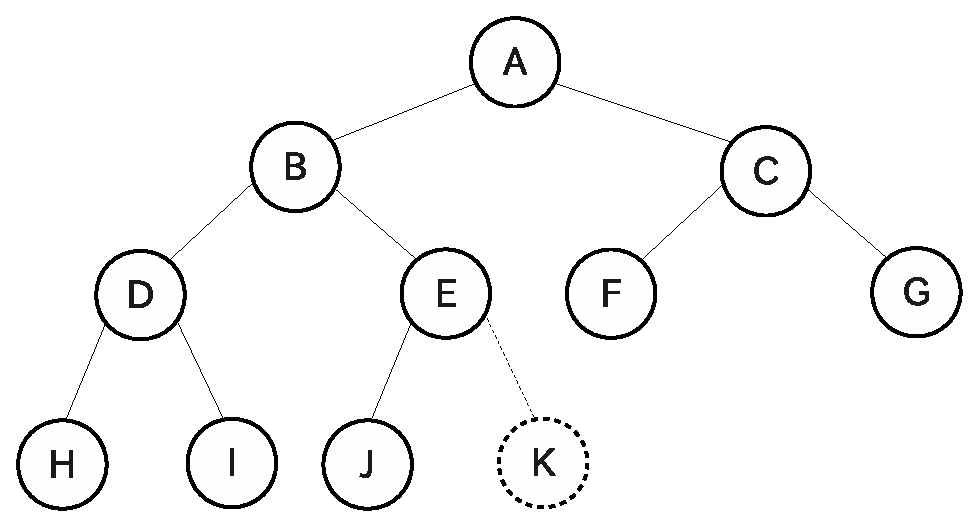
\includegraphics[width=0.8\linewidth,keepaspectratio]{fig13_4.eps}
\caption{ヒープの例(大小関係:アルファベット順に先に来るものが小さい)}\label{heap}
\end{figure}

なお、ヒープは親と子の大小関係については制約を設けているが、子同士の関係には言及していない点に注意しよう。すなわち、左側の子と右側の子の大小関係はどうでもいいのである。これは、二分ヒープに限らず、一般のヒープに言えることである。
\\ \\ 
図\ref{heap}のヒープは、確かに二つの制約を満たしている(そして同時に、偶然にも、左側の子ノードは右側の子ノードよりも小さい)。この関係性により、ヒープはソートや最小値/最大値を求める際によく用いられる。以下、この構築方法について記す。

\minisec{上方移動によるヒープへの要素挿入}
ヒープに新たな要素を加えることを考えよう。この時、図\ref{heap}のノードKのように、今埋まっていない階層の一番左側に新たなノードを追加する。これにより、shape propertyが保たれる。だが、単純に追加しただけではheap propertyが保たれない。

そこで、親ノードと比較し、順序が正しくない場合に親ノードと交換を行う\textbf{上方移動}\index{じょうほういどう@上方移動}(shift up)を行う。もしも、親ノードとの交換が起きた場合、再帰的にこれを実行し、交換が起きなくなるまで交換を繰り返す。これにより、追加ノードはヒープの適切な位置に挿入される。
\\ \\ 
何もない状態から、逐次上方移動によって要素を追加/挿入していけば、ヒープを構築することができる。

\minisec{下方移動によるヒープへの変換}
先程、最初のノードから順に上方移動で順次要素を追加していけばヒープを構築することができると記した。だが、これでは追加の度に再帰を行わなければならず、煩わしい。そこで\textbf{下方移動}\index{かほういどう@下方移動}(shift down)という操作を行い、全データの割り当てられた二分木をヒープへ変換する方法が知られている。
\begin{itembox}[l]{下方移動によるヒープへの変換}
前提として、全データをshape propertyを満たすように二分木に割り当てておく。
\begin{enumerate}
\item ヒープを後方(階層が深い側、同階層では右側)から順に見ていき「葉でないノード」を見つける。このノードを以下親ノードとする。
\item 見つかったノードに対し、子ノードと値を比較し、それらの最小値が親ノードの値となるように(必要に応じて)交換を行う。
\item 再び、最初のステップに戻り、探索を続ける。これを親ノード=根となるまで続ける。
\end{enumerate}
\end{itembox}

ここで紹介した上方移動/下方移動は、各々DFS/BFSと似た様相を呈している。木への操作の基本はDFS/BFSにあるため、再帰やキューといった道具を適切に使えるようにしておくと良い。

\subsection{二分探索木}
ヒープがソートに便利な木であったのに対し、\textbf{二分探索木}\index{にぶんたんさくぎ@二分探索木}(Binary search tree)はその名の通りサーチによく用いられる他、様々に応用がきく構造である。これは、二分木に対し、次の制約を課した木である。
\begin{itembox}[l]{二分探索木の制約}
任意の親ノードに対して
\begin{itemize}
\item その左側の部分木の全要素が、注目している親ノードの値と比べ小さいか等しい。
\item その右側の部分木の全要素が、注目している親ノードの値と比べ大きい。
\end{itemize}
という条件が成立すること。なお、ここでは等しいノードを左側に入れるとしたが、右側に入れても構わない(但し、木全体で左側に入れるか右側に入れるか統一されていなければならない)。
\end{itembox}

上記の制約のため、所定の値を検索する際に素早く検索できるのが二分探索木の特徴である。また、これに対して通りがけ順DFSで値を表示させた場合、昇順ソートされて値が出力される(もちろん、右側を先に持ってくれば降順ソートも可能である)。

\minisec{二分探索木の構築}
二分探索木に要素を追加するにはどうすればよいだろうか。これは、DFS同様に上側から順に見ていけば良い。ここで、注意しなければならないのは、ヒープの追加は下から上に木をたどっていったが、二分探索木では上から下にたどる、という点である。以下、具体的に手順を示そう。
\begin{itembox}[l]{二分探索木への要素の追加}
\begin{enumerate}
\item 最初に根ノードを「現在のノード」として以下の操作を行う。
\item 追加したい値が現在のノードよりも小さいか等しいならば左側へ、大きいならば右側へ進む。
\item 進んだ先にノードが存在しなければそこに追加したい値を新たなノードとして追加して終了する。ノードが存在する場合、そのノードを現在のノードとして、前項に戻る。
\end{enumerate}
\end{itembox}

これにより、最初に適当な根ノードを決め、これに対して順次要素を追加していけば二分探索木が構築できる\footnote{なお、この方法で構築していく時、例えば昇順/降順データが与えられたら、二分探索木は線形リストのような形になってしまう。これを防ぐために用いられるのが赤黒木などの平衡二分探索木である。本書では紙数の都合上扱わないが、興味があれば学んでみて欲しい。}。同様にして、二分探索木を用いてのサーチを行うこともできる。

\minisec{ノードの削除}
ここまではノードの追加/木の構築について話してきたが、必要なくなった要素は木から削除しなければならない。ヒープの場合、削除したい場所に最後のノードを移動し、大小関係について整合性を取れば良い(上方/下方移動)のであるが、二分探索木からの削除は少し面倒である。
\begin{itembox}[l]{二分探索木からのノードの削除}
\begin{enumerate}
\item 最初に根ノードを「現在のノード」として以下の操作を行う。
\item 現在のノードと、削除を行う値を比較する。この時、削除する値が現在のノードと等しければステップ4に進む。等しくない場合、削除する値が現在のノードよりも小さければ左側に、そうでなければ右側に移動し、次項へ進む。
\item 進んだ先のノードを現在のノードとして、前項へ戻る。
\item 現在のノードが子ノードを持たない場合はそのノードを削除して終了する。子ノードを持つ場合、削除した後に次項に進む。
\item 子ノードを1つだけ持つ場合は削除した場所を、子ノードによって置き換えて終了する。2つ持つ場合は削除したノードの右側部分木の最小値のノードで置き換える。この時、置き換え元(最小値)のノードに右側子ノードが存在するならば、右側子ノードを置き換え元ノードに置き換える(以下の関係は保つ)。
\end{enumerate}
\end{itembox}

\section{グラフ}
リンクリストは「前のノードが1つ・次のノードが1つ」というデータ構造であった。木は「前のノードが1つ・次のノードが複数」というデータ構造であった。この自然な拡張として、「前のノードが複数・次のノードが複数」というデータ構造を考えることができる。あるいは、前後の区別をなくし「隣り合ったノードが複数」という事もできる。路線図やロードマップ・地図のようなものがこのようなデータ構造をなしている。前後の区別をするならば、例えばロードマップの場合、一方通行の道路があったらそこには指向性がある。前後の区別をしないものとしては、例えば地図が考えられる。地図を見てみると兵庫県は京都府・大阪府・和歌山県・鳥取県・岡山県・徳島県・香川県と接しているが、これは接していることだけに意味があり、兵庫県から京都府へ方向付けする必要性はない。ここでは、「複数のノードが隣り合っているデータ構造」であるグラフを扱う。

\subsection{グラフの基礎概念}
\textbf{グラフ}\index{ぐらふ@グラフ}(graph)とは、\textbf{ノード}\index{のーど@ノード}(node,路線図でいう所の駅に当たるもの。日本語では\textbf{節点}\index{せつてん@節点|see{ノード}}ないし\textbf{頂点}\index{ちょうてん@頂点|see{ノード}}と呼ぶ。)とそれらをつなぐ\textbf{エッジ}\index{えっじ@エッジ}(edge,日本語では\textbf{辺}\index{へん@辺|see{エッジ}}。路線図でいう所の駅の間の線路に当たるもの。)からなるデータ関係をいう。図\ref{graph}にグラフの例を示す。

\begin{figure}[htb]
\centering
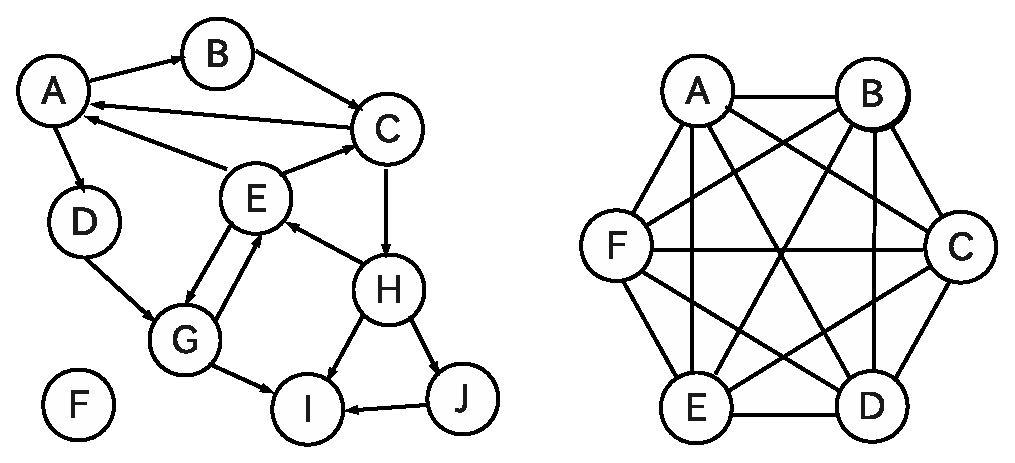
\includegraphics[width=0.9\linewidth,keepaspectratio]{fig13_5.eps}
\caption{グラフの例(左:有向グラフ・右:無向グラフ)}\label{graph}
\end{figure}

図\ref{graph}の左側のように、辺に指向性があるものを\textbf{有向グラフ}\index{ゆうこうぐらふ@有向グラフ}(digraph)と呼ぶ。これに対し、図\ref{graph}の右側のような、辺に指向性がないものは\textbf{無向グラフ}\index{むこうぐらふ@無向グラフ}(undirected graph)と呼ばれる。
\\ \\ 
グラフの各々の辺には方向づけを行うことができるが、それに加え\textbf{重み}\index{おもみ@(辺の)重み}を付けることができる。例えば路線図では、A-B間は3分、A-D間は2分、B-D間は4分などと所要時間を付けることができるが、この所要時間を辺毎にのせていけば、これが辺の重みになる。ここで挙げた路線図の場合は向きに寄って時間が変わったり一方通行だったりすることはないだろうが、ロードマップの場合は混雑の度合いによって所要時間がA→Bは30分、B→Aは25分などのように指向性を持つ場合があり、このような場合には有向グラフを用いることになる。ここでは重みを所要時間とした為、重みは正または0だろうが、実際には負の値を取る重みも存在する\footnote{負の値を取る重みなど、理論はともかく実際には何の役に立つのか?と思うかもしれない。だが、辺の途中でものの授受などがある場合は正負両方が必要だろう。例えば実生活でも、どこかに行く経路をたどる時、途中で銀行のある道でお金をおろすならば、その道ではお金がプラスになる。だが、お金を払わなければいけない道(有料道路など)があればお金はマイナスになるだろう。}。

\minisec{グラフの種類}
グラフには、その特徴に応じて幾つかの種類がある。ここではそれを紹介しておく。
\\ \\ 
無向グラフにおいて、任意の2ノード間に経路が存在するグラフのことを\textbf{連結グラフ}\index{れんけつぐらふ@連結グラフ}(connected graph)と呼ぶ。グラフを扱う場合、連結性を確かめてから使う場合が多い(チェックについては次項に述べる)。また、連結グラフでなくとも、適切な部分グラフに分ければ、連結グラフに分けて扱える。

図\ref{graph}右のように、全てのノードの間にエッジがあるようなグラフを\textbf{完全グラフ}\index{かんぜんぐらふ@完全グラフ}(complete graph)と呼ぶ。自己ループや多重辺(ある2ノード間に複数の同方向エッジが存在するもの)を含まない\textbf{単純グラフ}\index{たんじゅんぐらふ@単純グラフ}(simple graph)を扱うアルゴリズムを考える時、完全グラフはエッジの数が最大化されたグラフとして扱えるため、「エッジの多い場合の極端な例」としてしばしば用いられる。ノード数$V$の完全グラフに対して、そのエッジ数$E$は
\begin{equation}
E=\frac{V(V-1)}{2}
\end{equation}
により計算することができる。
\\ \\ 
また、閉路(ループ)を持たないグラフにも特別な名前が付いている。閉路を持たない連結グラフは、書いてみればわかるが、前述の木である。木をグラフとしてみた時、完全グラフとは逆にエッジ数が一番少ないため、「エッジの少ない場合の極端な例」として使うことができる。ノード数$V$の木に対してそのエッジ数$E$は
\begin{equation}
E=V-1
\end{equation}
である。

一方、閉路を持たない非連結グラフは、木が多く集まった形をなすことから\textbf{森}\index{もり@森}(forest)と呼ぶ。
\\ \\ 
以下では、無向単純グラフを基本に説明を行うこととし、単に「グラフ」と書いた場合は無向単純グラフを指すこととする。有向グラフの場合にも多少工夫することで同様のアルゴリズムを適用できる場合が多い。

\subsection{グラフの実装と連結性チェック}
ここでは、グラフを実装し、その連結性をチェックすることについて説明する。これは、グラフに関する諸問題の基礎となる部分である。
\minisec{隣接行列/接続行列による表現}
グラフを実装する場合、リストや木で用いたような構造体表現も可能であるが、重みやノード毎に個数が違う等の面倒な部分もある(有向グラフの場合は指向性の表現も面倒)。エッジ数が少ない場合は構造体表現も楽であるが、増えてきた場合(特に完全グラフの場合)は構造体表現は面倒である。そこで、グラフのノードを配列を用いて用意しておき、エッジに対し\textbf{隣接行列}\index{りんせつぎょうれつ@隣接行列}(Adjacency matrix)と呼ばれる行列を用いることが多い。

隣接行列は二次元配列を用いて実装される。隣接行列の\verb|[i][j]|成分をノード\verb|i|からノード\verb|j|への辺の重みとする。辺が存在しない場合は、それを表す値を代入しておく。重みがないグラフについては、1/0を辺の有無に対応させて用いる場合が多い。
\\ \\ 
また、別の実装として、ある点からある辺が出ているかどうかについて\textbf{接続行列}\index{せつぞくぎょうれつ@接続行列}(incidence matrix)を用いることもある。これは\verb|[i][j]|成分をノード\verb|i|からエッジ\verb|j|が出ているかどうかに対応させた行列である。単純グラフを扱う場合、この行列では1列にちょうど2個の1(ノードからエッジが出ている値)が見つかるはずである。

\minisec{グラフの連結性チェック}
グラフが連結であるかどうかは、アルゴリズムが適用できるかどうかを始めとして、様々な場面で重要である。ここではグラフの連結性を調べる方法について述べる。

グラフが連結であるということは、先に述べたとおり「任意の2ノード間に経路が存在する」ということである。ここで、無向グラフにおいてはある1ノードから全てのノードに到達可能である場合、他のノードからも全てのノードに到達可能であるという点に着目する。すると、ある1点から全ての点にエッジをたどって到達可能であるかどうかを調べれば良い、という結論に至る。
\\ \\ 
では、到達可能かどうかはどのように判定すればよいか。これは、実際にある1ノードから「もれなく・重複なく」たどってみれば良い。DFSないしBFSの出番である。各ノードが到達可能かどうかを表す一連のフラグ配列を用意し、これに可能であるかどうかを調べていけば良いのである。DFSを再帰処理で組むのは変わらないが、BFSの場合、キューを用いずとも、フラグ配列を順に見て行って、まだ見ていないノードを見れば良い。

同様に、連結性のチェックに限らず、グラフを探索する場合にはDFSかBFSのいずれかを用いるのが基本となる。
\\ \\ 
この後に話す最短路問題・閉路問題では連結グラフを前提とし、特段の記述がない場合非連結グラフは扱わない。

\subsection{最短路問題}
\textbf{最短路問題}\index{さいたんろもんだい@最短路問題}(Shortest path problem)とは、重み付きグラフにおいて、あるノードから別ノードへの道のうち重みを最小化するものを求める問題である。この内、ある2点間の最短路を求める問題は\textbf{2頂点対最短路問題}\index{にちょうてんついさいたんろもんだい@2頂点対最短路問題}と、単一の始点から全ての点への最短路を求める問題は\textbf{単一始点最短路問題}\index{たんいつしてんさいたんろもんだい@単一始点最短路問題}と、全ての点対について最短路を求める問題を\textbf{全点対最短路問題}\index{ぜんてんついさいたんろもんだい@全点対最短路問題}と呼ぶ。ここでは、図\ref{shortest}のグラフを例に、単一始点最短路問題と全点対最短路問題のアルゴリズムを紹介する\footnote{2頂点対最短路問題については、単一始点最短路問題のアルゴリズムを用いて求めれば良い}。

\begin{figure}[htb]
\centering
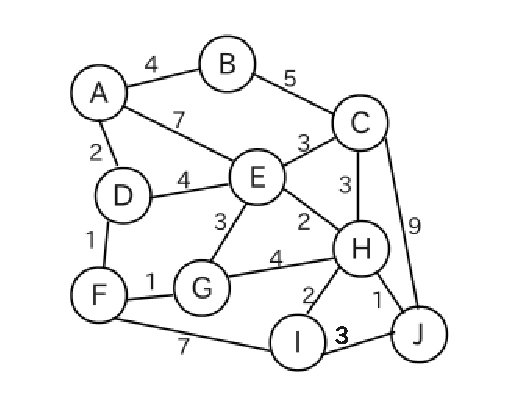
\includegraphics[width=0.5\linewidth,keepaspectratio]{fig13_6.eps}
\caption{重み付き無向グラフ}\label{shortest}
\end{figure}

なお、以下では最短路のコストを求めているが、最短路そのものを求める(経路復元)場合も同様のアルゴリズムで直前の頂点を記憶しておけば良い。もちろん、コストを求めてからBFS/DFSなどをしても求められる。

\minisec{Bellman-Ford法}
図\ref{shortest}の始点Aからの単一始点最短路問題を考えよう。ノード$i,j$を結ぶエッジの重みを$C_{i,j}$で表し\footnote{無向グラフの場合、$C_{i,j}=C_{j,i}$であるが、有向グラフでは区別する。また、ノード$i,j$間にエッジが存在しない場合、$C_{i,j}$は充分大きな値とする(実装では大きな値だが、理論上は$C_{i,j}=\infty$としても良い)。}、Aからノード$k$への最短距離(最小重み)を$D_k$として、次のような等式が成立する。
\begin{equation}
D_i=\min_j\left(D_j+C_{i,j}\right) \label{bellman}
\end{equation}

木の場合、式(\ref{bellman})を初期条件$D_A=0$の下で順次計算していけば全ての点への最短路が求められる。しかし、グラフに閉路が含まれる場合などは「順次」の順序を決めることができない。そこで、$D_A=0,D_{i(\neq A)}=\infty$として、式(\ref{bellman})を適用し、値を更新していく。この手法を\textbf{Bellman-Ford法}\index{Bellman-Fordほう@Bellman-Ford法}と呼ぶ。手順をまとめると次のようになる。
\begin{itembox}[l]{Bellman-Fordのアルゴリズム}
\begin{enumerate}
\item 初期化:スタートノードの値(最小コスト候補)を0、他のノードの値を$\infty$(充分大きな値)に設定する。
\item 各エッジに対して式(\ref{bellman})を適用して、その隣点からの最短距離更新がないかをチェックし、現在の「仮の最短距離」よりも小さければ更新する。
\item 前ステップを、更新がなくなるまで繰り返す。この反復は高々頂点数-1回で終わる。
\end{enumerate}
\end{itembox}

ノード数$V$、エッジ数$E$のグラフに対して、この時間計算量は$O(VE)$である。なお、時間計算量については次講か姉妹書の実習編を参照されたい。
\\ \\ 
負の重みを持つエッジ(有向グラフの場合は負の閉路)が存在した場合、最短経路は存在しない(その閉路を繰り返し通ることで無限に小さくできるため)。しかし、このケースでは、Bellman-Ford法が頂点数-1回の反復で終了しないため、それにより負閉路を検出することが可能である。これは、次に述べるDijkstra法にはない利点である。

\minisec{Dijkstra法}
Bellman-Ford法では、一度エッジを計算しても、その点への最短距離が定まるかどうかはわからなかった。そのため、更新を何度も繰り返した。だが、図\ref{shortest}のノードDへの最短路は、ノードAから出るエッジの重みなどを考慮すれば、$D_D=2$であると直ちにわかる。同様の論法で、$D_F=3,D_B=4,D_G=4$と、順次最短路を確定させていくことができる。そして、確定したノードへのエッジについては、もうこれ以上考慮に入れる必要はなくなる。これにより、Bellman-Ford法から無駄を省いた方法が次の\textbf{Dijkstra法}\index{Dijkstraほう@Dijkstra法}\footnote{このDijkstra(ダイクストラ)は構造化プログラミングの提唱者として知られているエドガー・ダイクストラその人である。}である。
\begin{itembox}[l]{Dijkstraのアルゴリズム}
\begin{enumerate}
\item 初期化:スタートノードの値を0、他のノードの値を未定義(または$\infty$)に設定する。
\item 確定ノードをピックアップできなくなるまで(=変化がなくなるまで)次の3,4のループを繰り返す。但し、最初の確定ノードはスタートノードとする。
\item 確定ノードから伸びているエッジをそれぞれチェックし、式(\ref{bellman})により現在の最小コストを計算し、そのノードの現在値よりも小さければ更新する。
\item まだ確定されていないノードのうち、最小の値を持つノードを見つけ、確定ノードとする(確定フラグを立てる)。
\end{enumerate}
\end{itembox}

Dijkstra法を図\ref{shortest}に適用した場合、確定ノードはA,D,F,(B,G),E,H,(C,J),Iの順に定まる。但し、括弧でくくったノードの順番は入れ替わることがある。
\\ \\ 
Dijkstra法は「現在の最小値はこれ以上更新されない」という考えに従うため、更新が起こりうる負のエッジを持つグラフ(有向・無向を問わない)については適用できない。また、ノード数$V$、エッジ数$E$のグラフに対して、Dijkstra法により最短路を求めるための時間計算量は$O(V^2)$である。ただし、これは確定ノードを決定する際に、ループを回して全てのノードをチェックするからであり、ここをヒープ(またはプライオリティーキュー)を用いて管理するとより速くなる。以下、これについて述べる。
\\ \\ 
スタートノードを根としたヒープを考えよう。ここでは簡単のため、図\ref{heap}の各ノードの文字と、図\ref{shortest}の各ノードの文字が対応していることにし、ヒープの各ノードには$D_i$の値を割り当てておくことにする。

ノードAに隣接しているノードを考えれば、$D_D,D_B,D_E$の更新が起こる。この更新を行った後、ヒープのノードAを削除する(削除方法は既に述べた)。そして根ノードとなったノードを確定ノードとし、同様の処理を施していけば良い。まとめると、次のようになる。
\begin{itembox}[l]{Dijkstraのアルゴリズム(ヒープ利用)}
\begin{enumerate}
\item 初期化:スタートノードの値を0、他のノードの値を未定義(または$\infty$)に設定する。
\item ヒープ初期化:最短距離の値についてのヒープを構築する。この際、ヒープのデータは、元のグラフのどのノードに対応しているかという事と、最短距離の値である。
\item ヒープのノードが尽きる(または1つになる)まで、次の4〜6の操作を繰り返す。
\item ヒープの根ノードに対応するグラフのノードを確定ノードとする。
\item 確定ノードから伸びているエッジをそれぞれチェックし、式(\ref{bellman})により現在の最小コストを計算し、そのノードの現在値よりも小さければ更新する。
\item ヒープから根ノードを削除し、更新した値を用いてヒープを再構築する。
\end{enumerate}
\end{itembox}

この方法を用いると確定ノードを速く決められる事になるため、時間計算量が$O(E\log V)$となる。これは、Bellman-Ford法に比べて速い方法である。そのため、最短路を定めることが可能な無向グラフや、負エッジを有しない有向グラフについてはDijkstra法が用いられることが多い。
\\ \\ 
なお、全てのエッジのコストが等しい場合には、単にBFSを用いてエッジ数を記録していったほうが簡単に経路を求められる。

\minisec{Warshall-Floyd法}
全点対最短路問題を解く場合には、各ノードに対する単一始点最短路問題をBellman-Ford法やDijkstra法により解いてもよいが、一般化した\textbf{Warshall-Floyd法}\index{Warshall-Floydほう@Warshall-Floyd法}を用いることが多い。この方法は、先の2つのアルゴリズムと違った漸化式を用いる(漸化式を作って計算する、\textbf{動的計画法}\index{どうてきけいかくほう@動的計画法}(Dynamic Programming,\textbf{DP}\index{DP|see{動的計画法}})の一種である)。

頂点に0-indexedにより番号をつける。第$k$番までの頂点及びノード$i,j$そのものを用いて構築可能な、ノード$i,j$間の最短経路を$D_{i,j,k}$と表すと、次の関係式が成立する。
\begin{equation}
D_{i,j,k+1}=\min(D_{i,j,k},D_{i,k+1,k}+D_{k+1,j,k}) \label{warshall}
\end{equation}
従って、この漸化式に対し、適切な初期値を定めて計算を実行すれば良い。初期値は
\begin{equation}
D_{i,j,0}=\min(C_{i,j},C_{i,0}+C_{0,j})
\end{equation}
とすれば良い(但し、$C_{i,j}$はノード$i,j$を結ぶエッジの重みで、存在しなければ$\infty$)。これをコードにまとめると次のようになる。なお、実際の実装の際には、$D_{i,j,k}$のうち、$k$を落としてしまって良い。
\begin{itembox}[l]{Warshall-Floydのアルゴリズムの実装}
\verb|i,j,k|はint型とし、式(\ref{warshall})に示したのと同じ意味を持つものとする。\verb|V|はグラフの頂点数で、\verb|D[i][j]|は$D_{i,j,k}$を表すものとする。また、\verb|C[i][j]|は隣接行列である。
\begin{lstlisting}[caption=Warshall-Floydのアルゴリズム,label=program13_3]
#define MIN(x,y) (((x)<(y))?(x):(y))

// initializing
  for(i=0;i<V;i++) for(j=0;j<V;j++) D[i][j]=MIN(C[i][j],C[i][0]+C[0][j]);
 
//calculation 
  for(k=1;k<V;k++) for(i=0;i<V;i++) for(j=0;j<V;j++)
                                        D[i][j]=MIN(D[i][j],D[i][k]+D[k][j]);
\end{lstlisting}
ここに示したコード断片により、\verb|D[i][j]|にノード$i,j$間の最短距離が入る。
\end{itembox}

ノード数$V$,エッジ数$E$のグラフに対して、Warshall-Floyd法は$O(V^3)$で動作する。Bellman-Ford法を全ノードに用いた場合$O(V^2E)$、Dijkstra法の場合$O(VE\log V)$であることを考えると、とりわけ、エッジ数が多いグラフに対して速いことがわかる。また、比較的実装が簡単なのも利点である。
\\ \\ 
さらに、Warshall-Floyd法は、負エッジを持つ有向グラフにも適用できる他、負閉路(無向グラフの場合負エッジ)の検出も可能である(\verb|D[i][i]|が負になる)。

\subsection{閉路問題}
グラフ理論の古典的な問題として閉路問題を紹介する。
\minisec{頂点の次数}
閉路問題の前に、ノードの\textbf{次数}\index{じすう@(ノードの)次数}という概念を導入する。各ノードに対し、それに接続しているエッジの数を次数と呼んでいる。有向グラフの場合、ノードに入ってくる辺の数を\textbf{入次数}\index{いりじすう@入次数}と、ノードから出ていく辺の数を\textbf{出次数}\index{しゅつじすう@出次数}と呼ぶ。

\minisec{オイラー閉路問題と一筆書き}
閉路問題は大きくわけて2つにわけられる。まず、全ての辺を1度ずつ通るような閉路である\textbf{オイラー閉路}\index{おいらーへいろ@オイラー閉路}(Eulerian cycle)について説明する。

与えられたグラフがオイラー閉路であるかどうか(このようなグラフを\textbf{オイラーグラフ}\index{おいらーぐらふ@オイラーグラフ}(Eulerian graph)と呼ぶ)は、次の定理により判定することができる。
\begin{itembox}[l]{オイラーグラフ}
与えられたグラフがオイラーグラフであることは、全ノードの次数が偶数であることと同値である。
\end{itembox}
\\ \\ 
オイラー閉路問題を言い換えると、スタート地点とゴール地点が同じ一筆書きでそのグラフを書くことができるかどうか\footnote{この問題の最も古典的な例として\textbf{ケーニヒスベルグの橋}が知られている。}の判定である。一方、現在よく考えられる一筆書きには、例えば数字の9のように、最初の点と最後の点が等しくないような場合もある。このような「一筆書き問題」の判定も考えてみよう。

一般に、一筆書き可能なグラフのことを\textbf{オイラー路}\index{おいらーろ@オイラー路}(Eulerian path)と呼ぶ。オイラー閉路は当然オイラー路でもある。オイラー路でありオイラー閉路でないようなグラフ(\textbf{準オイラーグラフ}\index{じゅんおいらーぐらふ@準オイラーグラフ}(semi-Eulerian graph))は、次のように判定できる。
\begin{itembox}[l]{準オイラーグラフ}
与えられたグラフが準オイラーグラフであることは、全ノードのうちに次数が奇数であるものがちょうど2つ存在する事と同値である。
\end{itembox}

以上から、一筆書き可能かどうかは、グラフにおいて全ノードのうち、次数が奇数であるものが存在しないか2つ存在するかによって判定可能である。なお、オイラーグラフの始点(=終点)はどこでもよいが、準オイラーグラフの始点と終点は、次数が奇数である2つのノードである。

\minisec{ハミルトン閉路問題と巡回セールスマン問題}
オイラー閉路が全辺を通る問題だったのに対し、\textbf{ハミルトン閉路}\index{はみるとんへいろ@ハミルトン閉路}(Hamiltonian cycle)は全ての頂点を1度ずつ通るような閉路の事を言う。閉路でないが全ての頂点を1度ずつ通るような路を\textbf{ハミルトン路}\index{はみるとんろ@ハミルトン路}(Hamiltonian path)と呼ぶのは、オイラー路と同様である。

与えられたグラフが、ハミルトン閉路を\underline{含む}場合、そのグラフを\textbf{ハミルトングラフ}\index{はみるとんぐらふ@ハミルトングラフ}(Hamiltonian graph)と、ハミルトン路を含むがハミルトン閉路を含まないグラフを\textbf{準ハミルトングラフ}\index{じゅんはみるとんぐらふ@準ハミルトングラフ}(semi-Hamiltonian graph)と呼ぶ。オイラーグラフはグラフそのものであったが、ハミルトングラフは含むかどうかである点に注意されたい。
\\ \\ 
あるグラフがハミルトングラフであるかどうか判定するハミルトン閉路問題を効率よく解くアルゴリズムはない。ハミルトン路を含むかどうかの判定は、それ以上に難しいとされる。さらに、ハミルトン閉路問題に重みをつけた、「ハミルトン閉路のうち最短路を求めよ」という問題は\textbf{巡回セールスマン問題}(Traveling Salesman Problem,\textbf{TSP})として知られる難問である。ハミルトン閉路問題はClass-NP(後述)に属するが、ハミルトン路問題や巡回セールスマン問題はClass-NPにすら属さない(丸つけすら難しい)可能性のある問題であり、オイラー閉路同様に古典的であるが、難易度は雲泥の差である。
\\ \\ 
ここまで、グラフについて古典的な問題を扱ったが、グラフの問題には、彩色問題・マッチング・フロー問題・最小全域木など、まだまだ多くの問題が存在する。詳しくはグラフ理論の専門書\footnote{例えば、「シリーズ 情報科学の数学 グラフ理論」(恵羅,土屋 1997 産業図書)などがある。}を参照されたい。

\newpage
\begin{shadebox}
\section*{本講の要点}
本講では、データを適切に整理して扱うために、基本的なデータ構造を学んだ。
\subsection*{基本的なデータ構造}
\begin{itemize}
\item スタックはLIFO、キューはLILOのデータ構造である。
\end{itemize}

\subsection*{リンクリスト}
\begin{itemize}
\item リンクリストは、ポインタを用いてデータの順序関係を示し、データの挿入や削除を容易にしたものである。
\item リンクリストの各要素は最大1つまでの前要素/次要素を持つ。
\item リンクリストを実装する場合には自己参照構造体を用いる。
\item リンクリストに循環が存在するかどうかは、2つのポインタを「おいかけっこ」させることにより判定できる。
\end{itemize}

\subsection*{木}
\begin{itemize}
\item 木構造は前要素を1つ以下、次要素を複数持つデータ構造である。
\item 任意の木は、前要素1つ以下、次要素2つ以下の二分木に変換できる。
\item 木の探索(走査)方法はDFSとBFSが知られている。
\item ノード間あるいは木全体に制約をかけることで、ヒープや二分探索木といった様々な木を実装できる。
\end{itemize}

\subsection*{グラフ}
\begin{itemize}
\item グラフは前要素・次要素ともに複数持つデータ構造である。前後の区別をなくしたものもある。
\item グラフが連結しているかどうかは様々な問題の基礎になる。連結の判定はBFSやDFSによる。
\item 重み付きエッジを持つグラフに対し、そのノード間の最小重みを求める問題を最短路問題と呼んでいる。最短路問題にはBellman-Ford法・Dijkstra法・Warshall-Floyd法などの方法が知られている。
\item 閉路問題は大きくオイラー閉路とハミルトン閉路に分かれる。前者は次数を数えることで判定可能であるが、後者は簡単には解けない。
\end{itemize}

\end{shadebox}
